\chapter{Formal Project Proposal}

\begin{TempText}
	(Max 10 pages)
\end{TempText}

\begin{TempText}
	@Note: Use this chapter for Rough Draft Proposal/Final Proposal 
\end{TempText}

\begin{TempText}
	@Note: A formal game proposal makes up the first chapter of your project notebook. The game proposal describes your game idea, provides a detailed development schedule, and gives a qualitative assessment of your project. The proposal should be professionally prepared, expressive, grammatically sound, illustrative of your efforts and process, and easy to understand. A good design effort can easily be hampered by a poor communication of what was done	
\end{TempText}

% ====================================================================================

\section{Game Description}

\subsection{Overview}

\begin{TempText}
	@Note: What is the genre of your game? Is it a 2D or 3D game? Is it a single player or multiplayer game? Explain the main goal of the game and/or the main purpose to be achieved by players. 
\end{TempText}

\begin{TempText}
	@Important: You need to design a project whose complexity fits the timeline of the course and the skills of your group.
\end{TempText}

\begin{TempText}
	@Important: Your game needs to really stand out in one way, but not all ways. Doing one aspect of it well will get you a better grade than doing a mediocre job on a lot of things.
\end{TempText}

We are developing a 2D, round-based, local multiplayer, semi-cooperative platformer race game. The main goal of the game is to navigate a maze-like decrepit tower structure and escape the rapidly rising mountain of quicksand piling up at the below. The game is round-based where the rounds are fast-paced bursts of cooperation, betrayal, and action. A player wins after a culmination of rounds by obtaining the highest score via escapes and collectibles overall.

A player who is too slow to climb or stands on the rising sand for a time, gets stuck in it and is engulfed. That player looses the round and joins the game again at the start of the next round.

The players are engaged in a race to the top as escaping first is the main objective of each round and gives the player the bonus of first-choice in an in-between-round item shop. While there are items to collect during the level, these have relatively minor effects/power ups/buffs compared to those which are found in the round-shop.

Each item can be used both cooperatively and/or adversarially. For example, with a ``chain-fling'' item, a player can prevent another player from reaching the top by pulling them down, or help another player by flinging them up.

Each level has a number of small built-in challenges which require one or more players to complete. They are simple to understand and quick to complete, and have a boon for completing them (e.g., items or currency). The idea being that completing a challenge requires cooperation but can also lead to betrayal by players. For example, one challenge might require a group of players to stand on a specified platform for the platform to activate and quickly move upwards. But if one player jumps off the platform during its accent, the platform breaks, leaving those who chose not to jump off to fall and recover.

\subsection{Background Story}

We currently have a few possible direction to take the storyline. Which one we choose will largely depend on the finer details of the gameplay.

\subsubsection{Grave Robbers}

The players play as a band of grave robbers, plundering a series of burial towers in the desert. Whenever they enter a tower, it starts sinking into the sand and they have to scramble to the top to get out while grabbing as much treasure on their way. The grave robbers are fiercely competitive and not exactly loyal and work together only when they stand to benefit themselves and will gladly throw each other under the bus if they think it will help them get their hands on more gold.

A shaman appears to be following them around from tower to tower, selling the robbers magical items to help them brave the traps in the towers as well as betray their companions. The shaman seems uninterested in gold and only accepts strange gems that can be found in the towers and seem worthless to the robbers.

\subsubsection{Desert Shopaholics}

The spaceship drops you, alien shopaholics, here in the earth's desert where golds and gems are hidden deep in the sand. More importantly, there are many shops! However don't forget that shopping is forbidden in your planet and you have been targeted by the shopping police. They already located you in the tunnel and decided to cause you some trouble.(*Or simply: However, the tunnel is not that firm and because of your brutal exploring, it starts to falling apart. ) Sands are gushing out from all direction. Time is limited, all you want to do is to grab each penny in your sight and head to the shops one by one before your life is threaten. Besides, You wouldn't stand that your buddy reach to the shop before you do, because you know you only want the BEST and the RAREST earth goods.


\subsubsection{Mummy Escape}

The players are mummies awoken by an archaeological activity. When they open their eyes, they see stupid human have triggered the curse mechanism, and the tomb is falling apart. While they're escaping for a second chance at life, they mustn't forget to grab the treasures. According to some prophesy only one of you can be back to the ground.


\begin{TempText}
    
    
    
	@Note: Describe any background or storyline associated with the game.
\end{TempText}

\subsection{Design Decisions}

\begin{TempText}
	@Note: Here describe the core mechanics of your game, gameplay features, and visual style. What makes the game interesting and fun? While writing your design choices, don't forget to explain the reasons behind and how they follow the theme. Put mocked-up screenshots and/or sketches. Pencil sketches are fine. You don't need beautiful artwork at this point. You can also discuss how the controls are set up and whether it should support an Xbox controller as an input method.
\end{TempText}

The game is designed to be played as a group of 2-6 players using gamepad controllers as the input method.

\begin{figure}
    \centering
    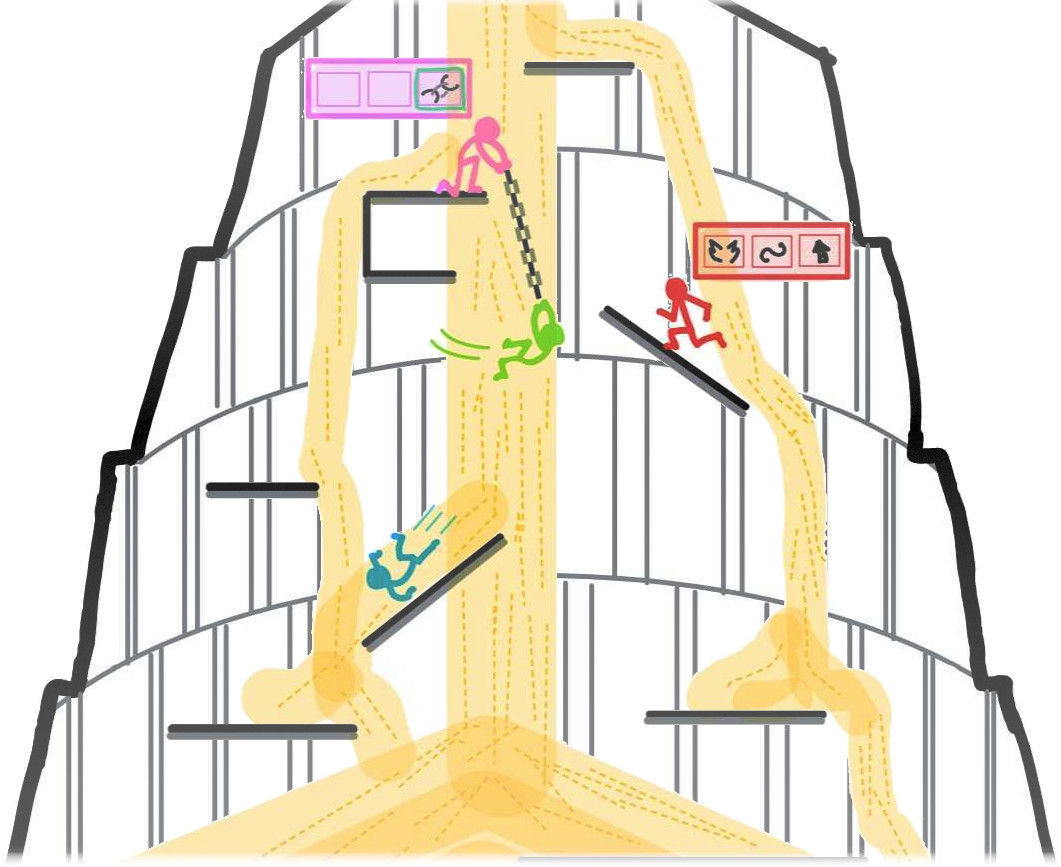
\includegraphics{figures/topmeifyoucan_concept.jpg}
    \caption{Concept of four players racing to the top with one falling due to sand, and others using an item cooperatively.}
    \label{fig:concept}
\end{figure}

The core mechanic of our game is the rising sand-mountain which acts as the main antagonistic force of the game, swallowing players as they fall into it. This forces the players to keep moving upwards and makes trying to loot the entire tower impossible, thereby putting pressure on the players when making decisions. The sand is falling from the top of the tower, flowing along platforms and (maybe) interacting with the player.

To add to this, players will have access to items which enable player interaction. It is up to the players to form alliances or rivalries, the items will help you do either.

\begin{figure}[h]
    \centering
    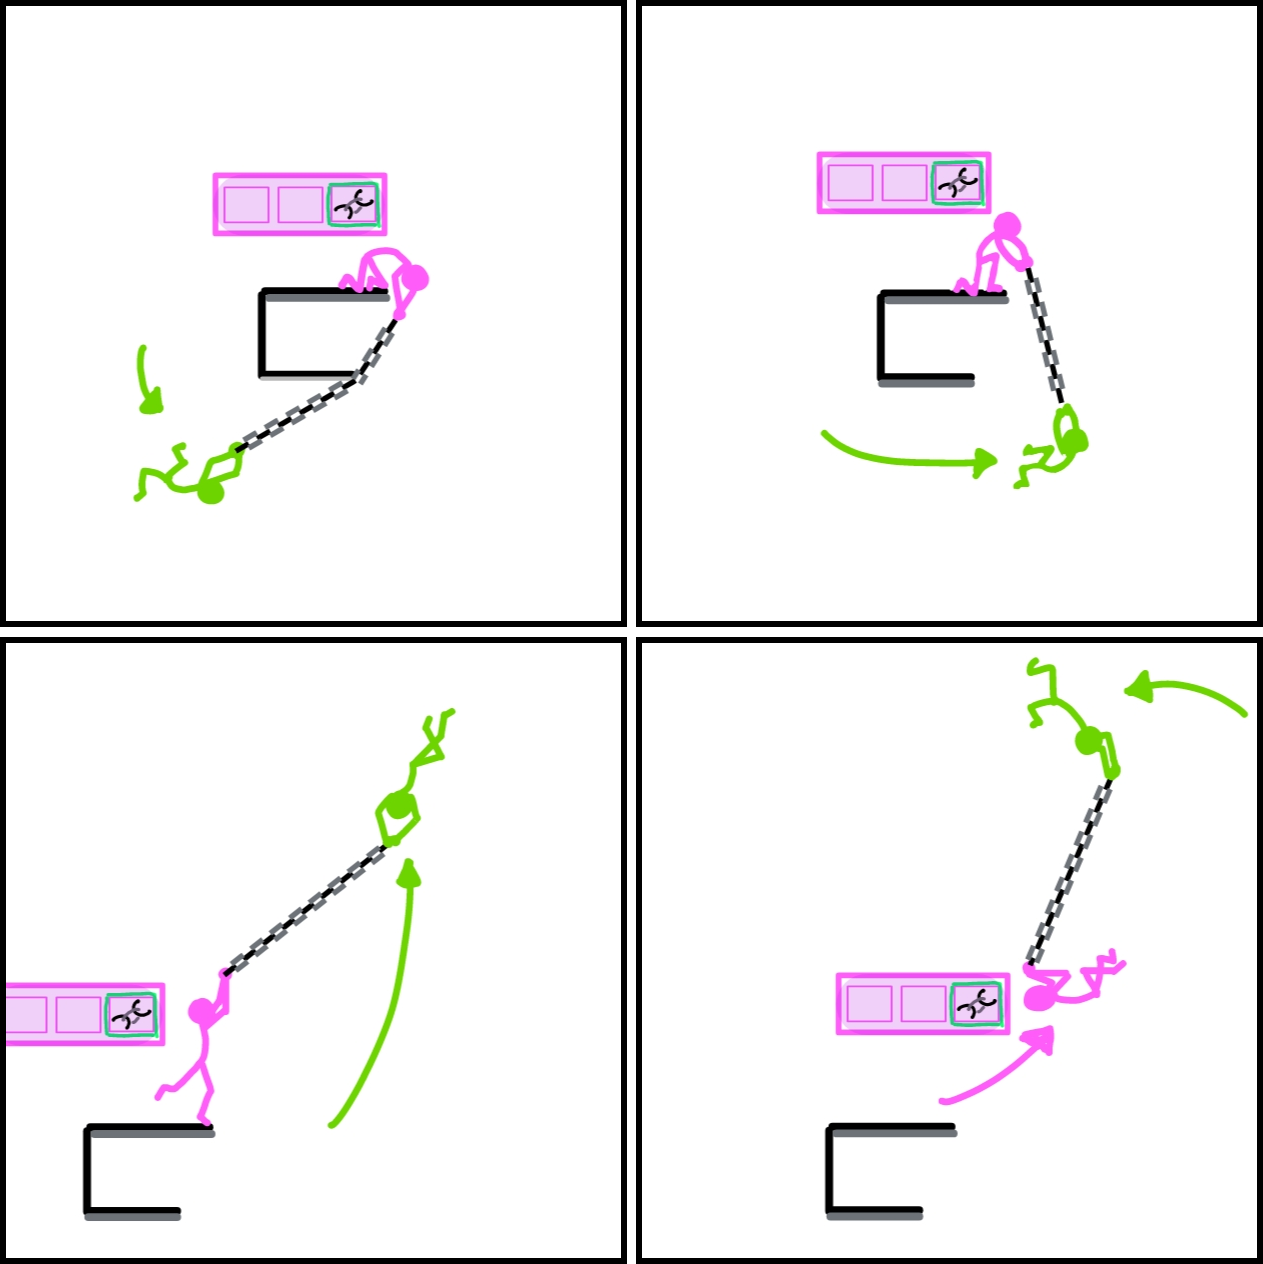
\includegraphics[width=0.5\textwidth]{figures/topmeifyoucan_concept_rope_coop.png}
    \caption{Concept of two players using an item cooperatively.}
    \label{fig:concept-coop}
\end{figure}

\begin{figure}[h]
    \centering
    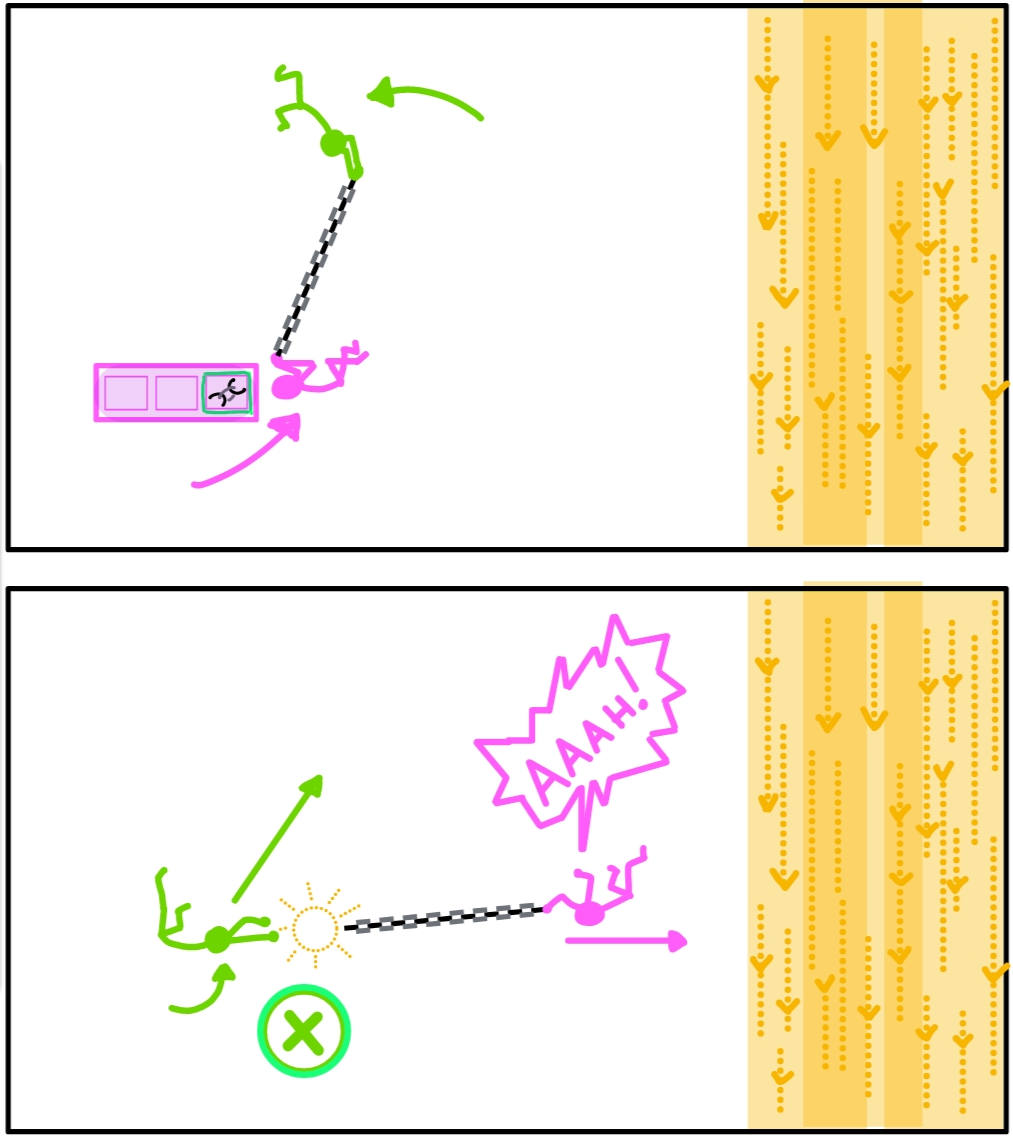
\includegraphics[width=0.5\textwidth]{figures/topmeifyoucan_concept_rope_betrayal.png}
    \caption{Concept of a player using an item adversarially. One player releases the chain to fling the other into a downward sand stream.}
    \label{fig:concept-betrayal}
\end{figure}

The main fun-factor of our game is the unpredictability of each round. the forming and breaking of alliances will keep the players on the edge of their seats as they scramble to reach the top. While the platforming action is the main appeal, the game also provides abundant opportunities for planning. ``Do I just rush past these coins and get ahead, or spend time collecting then for a better item which will help me later in the game?'' Of course, other players can and will put and end to your plans which adds depth to the concept.

The game will have 2D sprite graphics inspired by architectural styles.




% ====================================================================================

\section{"Big Idea" Bullseye}

\begin{TempText}
	@Note: Highlight the primary, central, most important conceptual idea of your game, as well as the central, supporting, extra-special and impressive technical component. Your entire team should agree upon and buy into these two concepts during the design phase so that everything that goes into the project is focused and aligned around a common and unified goal. It sounds a bit obvious, but it's a powerful tool.
\end{TempText}

\begin{TempText}
	@Note: Include a graphic big idea bullseye in your game proposal. The primary and secondary drives should be short, direct, and to the point.
\end{TempText}

The bullseye of our game is the social aspect we are trying to achieve. The game will give tools for the player to cooperate and play against one another while ultimately only allowing one winner. Therefore we are expecting alliances of varying durations to from during the game only to be broken at the latest by the end of the game.

The technical components facilitating this will be mini challenges strewn throughout the levels which require multiple players to overcome, but provide ample opportunities for betrayal, as well as the collection of small items and power ups and the input-control design.

% ====================================================================================

\section{Technical Achievement}

\begin{TempText}
	@Note: Your game should include at least one core technical item. This technical element should help your game stand out in an innovative way by providing an element that goes beyond the normal functionalities. This is your chance to select a concept from another course or something that you have always been interested in and implement it in the context of your game. Try to impress us, while still ensuring that the concepts you target fit within the scope of the course.
\end{TempText}

\begin{TempText}
	@Note: This section should detail the core technical item you plan to include. You are free to present more than one idea, but remember that it's better to be super successful at one item than to try to include many and fail.
\end{TempText}

We plan on the technical achievement of our game to be one of the following.

\begin{itemize}
    \item Dynamic Sand Simulation. Sand is flowing down the level and interacting with players.
    \item A power-up which is particularly challenging to implement, like a rope connecting two players with a diverse range of physics.based applications.
    \item Procedural/Infinite Level generation
\end{itemize}

% ====================================================================================

\section{Development Schedule}

\begin{TempText}
	@Note: The development schedule is crucial and should contain two basic parts. First, you must provide a layered development description of your game that divides the development schedule into five categories based on how crucial each element is. Second, you must provide a timeline for the course including major milestones and deliverables.
\end{TempText}

\begin{TempText}
	@Note: Structure your development so that you complete each layer before going on to the next. Plan exactly what is entailed in each layer, and which team member is going to do each component. Include this layered description in your proposal.
\end{TempText}

\subsection{Layered Task Breakdown}

\begin{TempText}
	@Note: You can't accurately anticipate how long each step in your project is going to take. Consequently, you need to make a detailed development schedule that is layered.
\end{TempText}

The following list presents the different targets that our team aims to achieve, and gives a short description of what each of them contains. We are still in the process of breaking some of these down into concrete work packets.

\subsubsection{Functional Minimum}

\begin{TempText}
	@Note: Minimal items to make something that you might call a game. You'd be embarrassed if you only got this far, but at least it'd be something.
\end{TempText}

The functional minimum is a single-player platforming experience. It includes at least one level where the player jumps from platform to platform. The controls and the collision detection need to be implemented.

\subsubsection{Low Target}

\begin{TempText}
	@Note: Your target for what you want to get done--the least possible to feel sort-of OK about the result.
\end{TempText}

The low target is a local multiplayer game, which uses gamepads. The game is expected to be played by a group of friends at a party, so the rounds will be kept up to at most 4-5 minutes long.
    
The aim of the players is to race to the top of the level, while sand is rising from the bottom. Touching the sand kills the players. The first player to reach the top wins the round.
    
Unlike the functional minimum, the players will be animated. This will improve the visual aesthetic of the game and make it more appealing.

\subsubsection{Desired Target}

\begin{TempText}
	@Note: This is what you're aiming for, if things go reasonably well.
\end{TempText}

In addition to winning the round, the desired target will include conditions to win the game overall. This can be the conclusion of the overarching story of the game, with the winner being clearly shown and congratulated for their achievement by a win screen.

The game will involve buying of items between rounds. Those items will be bought by players with money that will be collected during the level and at the end of each round based on the order in which they finish. Those items can be used to more easily win subsequent rounds, such as speed boosts, power boosts and so on.

The game will additional have small challenges in the rounds. Those challenges would involve a simple puzzle that may require the collaboration of more than one players. Those challenges will not be mandatory to complete the round, but will give the player additional coins or items.

\subsubsection{High Target}

\begin{TempText}
	@Note: It might be possible to get this much done, if all goes extremely well.
\end{TempText}

The high target will further include breakable sand platforms, which will break after a given set of seconds upon standing on them.

Each round will begin with a starting challenge, that needs to be completed by all players in collaboration before the sand starts rising and the timed part of the game commences.

Additionally, a ranking for the players and statistics for each round will be shown in the end.

The shop will further include additional items to buy.

\subsubsection{Extras}

\begin{TempText}
	@Note: Stuff that you know you can't get done this semester, but you might add later if you decide your game is cool enough to keep working on after the class is over, just for fun.
\end{TempText}

Additional rubber banding for the weakest players, so that they continue playing and having fun.

Additionally, sand will be falling from the top to the bottom throughout the levels, which will interact with the player and slow them down or kill them.

A player can trap another player via the cage item. The player can stay close to the cage they have dropped in order to make it last longer.

A binding mechanic which allows players to attach to each other and help with the completion of the levels. The players can choose to detach themselves from each other after a given period of time has passed.

Mini boss fights inside the rounds, in which the players are forced to collaborate in order to succeed.

Items can hit the players while they race to the top, which slows them down or kill them.

\subsection{Task List}

% draw art assets, 
% animation,
% level design,
% audio,
% player control,
% game engine,



\begin{TempText}
	@ Note: Provide a table showing who is responsible for each task, how many hours will each task require, etc.
\end{TempText}




\subsection{Timeline}

\begin{TempText}
	@ Note: Provide a Gantt chart when each task will be started and finished, etc.
\end{TempText}

% ====================================================================================

\section{Assessment}

\begin{TempText}
	@Note: Tell us what the main strength of the game will be. What part is going to be the coolest? Who might want to play this game? What do they do in the game? What virtual world should the system simulate? Basically, you are setting up a world view for your subsequent design. What criteria should be used to judge if your design is a success or not?
\end{TempText}

